%!TEX root = ../main.tex
\section{Homework \thesection}


\subsection{Fitting Curves with Linear Least Squares}
We discussed the least-square formulation for a slope-intercept model of a line during lecture.
\begin{equation}\label{linearregression}
E(m, b)=\sum_{i=1}^{n}[y_i-mx_i-b]^2
\end{equation}
And we also talked about fitting a quadratic curve using LLS.
Now, assume you got some sample points from some experiments, i.e., \href{./hw1/problem1/hw1_p1.mat}{\texttt{hw1\_p1.mat}} in the problem1 folder.

\begin{enumerate}
	\item Say you want to fit the data to a cubic curve.
	Write down the least squares formulation (in a form similar to Eq.\ref{linearregression}) as well as the matrix formulation of it.
	Explain why this problem could be solved by using Linear Least Squares despite the fact that the curve is non-linear.
	\item Implement the solution of the LLS problem you wrote in (1).
	Report resulting coefficient values and a plot of the fit;
	include your code verbatim in your pdf submission.
	The file named \href{./hw1/problem1/viz_curve.m}{\texttt{viz\_curve.m}} will plot the curves for you.
	Increase the order of curves, such as 4,5 and 6, and report their resulting plots as well.
	\item Does the curve with higher orders fit the data better?
	Explain what you observe.
\end{enumerate}


\subsubsection{Cubic model}
The least squares formulation of cubic curves is
\begin{equation}
E(b_3,b_2,b_1,b_0)=\sum_{i=1}^{n}\left[y_i-\left(b_3 x_i^3 + b_2 x_i^2 + b_1 x_i + b_0 \right)\right]^2.
\end{equation}
Linear Least Square does not mean the curve needs to be linear.
Here, linear means that the response should be a linear combination of predictors.
As long as the predictors are linearly independent, we can always use the Linear Least Square method.
The key point is to define a proper set of predictors.
From linear algebra, we know that polynomials with different degrees are independent.
Since cubic curves have degree at most 3, the set of linearly independent polynomials has dimension 4.
For simplicity, we do not require the basis to be orthogonal.
Instead, we take the simpliest basis: \(x^3, x^2, x, 1\).
The Least Square method is to determine the linear combination that minimize the sum of square errors.
If written in matrix form,
\begin{equation}
\begin{bmatrix}
y_1 \\ y_2 \\ \vdots \\ y_n
\end{bmatrix}
=
\begin{bmatrix}
x_1^3 & x_1^2 & x_1 & 1 \\
x_2^3 & x_2^2 & x_2 & 1 \\
\vdots & \vdots & \vdots & \vdots \\
x_n^3 & x_n^2 & x_n & 1
\end{bmatrix}
\begin{bmatrix}
b_3 \\ b_2 \\ b_1 \\ b_0
\end{bmatrix}
+
\begin{bmatrix}
e_3 \\ e_2 \\ e_1 \\ e_0
\end{bmatrix},
\end{equation}
or equivalently,
\begin{equation}
Y=Xb+e.
\end{equation}
And the sum of square error is
\begin{equation}
E(b_3,b_2,b_1,b_0)=e^Te
\end{equation}
According to the result from multilinear regression, the best \(b\) that minimize the square error is
\begin{equation}
b=\left(X^T X\right)^{-1}X^TY
\end{equation}

\subsubsection{Implementation}
The implementation is very short.
And I tried the increased order of curves, up to order 7.
The code and plots (Figure \ref{fig:1}) are listed below.
\begin{lstlisting}[style=Matlab-editor]
x=[X.^3 X.^2 X.^1 X.^0]
C3=inv(x'*x)*x'*Y
x=[X.^4 X.^3 X.^2 X.^1 X.^0]
C4=inv(x'*x)*x'*Y
x=[X.^5 X.^4 X.^3 X.^2 X.^1 X.^0]
C5=inv(x'*x)*x'*Y
x=[X.^6 X.^5 X.^4 X.^3 X.^2 X.^1 X.^0]
C6=inv(x'*x)*x'*Y
x=[X.^7 X.^6 X.^5 X.^4 X.^3 X.^2 X.^1 X.^0]
C7=inv(x'*x)*x'*Y
viz_curve(C3,X,Y)
viz_curve(C4,X,Y)
viz_curve(C5,X,Y)
viz_curve(C6,X,Y)
viz_curve(C7,X,Y)
\end{lstlisting}

The coefficients are
\begin{equation}
\begin{bmatrix}
b_3 \\ b_2 \\ b_1 \\ b_0
\end{bmatrix}
=
\begin{bmatrix}
	-0.00866565736949468\\
	-0.205773475198218\\
	2.34336989430312\\
	1.26227984182860
\end{bmatrix}
\end{equation}


\begin{figure}[htbp]
	\centering
	\begin{subfigure}[t]{0.5\textwidth}
		\centering
		\includegraphics[width=\textwidth]{hw1/problem1/f1.pdf}
		\caption{Order 3}\label{fig:1a}
	\end{subfigure}

	\begin{subfigure}[t]{0.42\textwidth}
		\centering
		\includegraphics[width=\textwidth]{hw1/problem1/f2.pdf}
		\caption{Order 4}\label{fig:1b}
	\end{subfigure}
	\quad
	\begin{subfigure}[t]{0.42\textwidth}
		\centering
		\includegraphics[width=\textwidth]{hw1/problem1/f3.pdf}
		\caption{Order 5}\label{fig:1c}
	\end{subfigure}
	\begin{subfigure}[t]{0.42\textwidth}
		\centering
		\includegraphics[width=\textwidth]{hw1/problem1/f4.pdf}
		\caption{Order 6}\label{fig:1d}
	\end{subfigure}
	\quad
	\begin{subfigure}[t]{0.42\textwidth}
		\centering
		\includegraphics[width=\textwidth]{hw1/problem1/f5.pdf}
		\caption{Order 7}\label{fig:1e}
	\end{subfigure}
	\caption{Linear Least Square fit on models of different orders}\label{fig:1}
\end{figure}



\subsubsection{Observation and discussion}
In general, \emph{if the sum of square error is the rubric to evaluate the fitness, then the higher the interpolation order, the smaller the sum of square error, which indicates the better fitness.}
This is because the higher order interpolation has more coefficients to minimize the errors at each \(x_i\).
The extreme case is the number of coefficients equals to the number of data points, which leads to perfect interpolation and no errors.

However, it seems from Figure \ref{fig:1a} that the cubic curve follows the trend of the points quite well.
In comparison, when the order increases, the trend becomes wired, although the curve seems to be closer to every point.
This shows that curve with higher orders may not fit the data better, which may be called as \emph{overfit}.
And when the order reaches 7, MATLAB shows the warning ``Matrix is close to singular or badly scaled. Results may be inaccurate.'' and provide the condition number of \(X^T X\) is 8.4867e+17, which means it is nearly singular.
Furthermore, the round-off error due to the precision limit of MATLAB will cause a relatively large error.



\subsection{Lambertian Model}
Recall the Lambertian model of reflectance:
\begin{equation}\label{lambertian}
R(x) = \rho l(x)^T n(x)
\end{equation}
\begin{enumerate}
	\item There are two people standing at location A and B.
	Who will observe stronger reflection at point x? Why?
	\item Tell one drawback of Lambertian model and name a specific object in the real world whose reflectance is not well modeled by the Lambertian model.
\end{enumerate}

\subsubsection{Reflection intensity}
Since the reflection intensity only depends on \(\rho\) and \(x\), it is the same for both observers.
% Recall that any reflected light intersecting an image plane, by way of a camera projection function \(P\), would induce a perfect image:
% \begin{equation}\label{perfectimage}
% \mathcal{I}(u)=P(R(x))
% \end{equation}
% We can observe that for a fixed \(R(x)\), the projection on the B's plane is shorter than the one on A's plane.
% This means that the intensity of refection observed by B is greater than the one by A.
% So B observes a stronger reflection.

\subsubsection{Drawback of Lambertian model}
The practical drawback of Lambertian model is that it is too simple (sometimes naive).
It only gives the intensity of reflection as a scale.
It cannot describe the easiest case -- mirror reflection -- in physics.

Mathematically, this model will fail when the normal vection \(n(x)\) is not defined.
In 3 dimensional case, the normal vector can be obtained by the cross product of two linearly independent tangent vector, and the tangent vectors can be defined by the partial derivatives.
So if the surface is not differentiable, the Lambertian model will fail.
For example, the edge of a knife, the point of a needle or the boundary of a Koch snowflake.




\subsection{Bayer Demosaicking}
To digitalize a perfect color image, we overlay the Bayer pattern filter on top of the photo sensors to accept RGB separately.
We could call this process mosaicking.
Assume that you've got a digital image filtered by the Bayer pattern and want to demosaic it, i.e., reconstruct the original color image.
One of the common ways to do this is to use bilinear interpolation.
For a green pixel, two red neighbors can be interpolated to yield the red value and two blue neighbors can be interpolated to yield the blue value, and similar for red or blue pixels.
The only difference is that for red or blue pixels you need to consider 4 neighbors instead of 2.

In Matlab, the function \texttt{demosaic} actually does this job, but now you need to implement this function by your own.
Pick any color image you like and use bayer filter.m to generate a Bayer encoded image.
Implement the demosaicking algorithm in \href{./hw1/problem3/mydemosaic.m}{\texttt{mydemosaic.m}}.
Report the original image, filtered image and reconstructed image; include your \href{./hw1/problem3/mydemosaic.m}{\texttt{mydemosaic.m}} verbatim in your pdf submission with brief explanation.
Submit your code together with your report.

\lstinputlisting[style=Matlab-editor]{./hw1/problem3/mydemosaic.m}

The code listed above with some comments is the implementation of \href{./hw1/problem3/mydemosaic.m}{\texttt{mydemosaic.m}}.
Most of the code (loops and if-else cases) deals with the boundary conditions, since MATLAB will report overflowed index on the boundary if we forget to check.
The result is quite satisfying.
I use an image that I took personally at the Palace of Fine Arts in San Francisco.
Three standard size photos were taken and stinched together to create Figure \ref{fig:2}.



\begin{figure}[htbp]
	\centering
	\begin{subfigure}[t]{\textwidth}
	    \centering
		\includegraphics[width=0.95\textwidth]{hw1/problem3/homepage.jpg}
		\caption{Original image}\label{fig:2a}
	\end{subfigure}
	\begin{subfigure}[t]{\textwidth}
	    \centering
		\includegraphics[width=0.95\textwidth]{hw1/problem3/gray.png}
        \caption{Filtered image}\label{fig:2b}
	\end{subfigure}
	\begin{subfigure}[t]{\textwidth}
	    \centering
		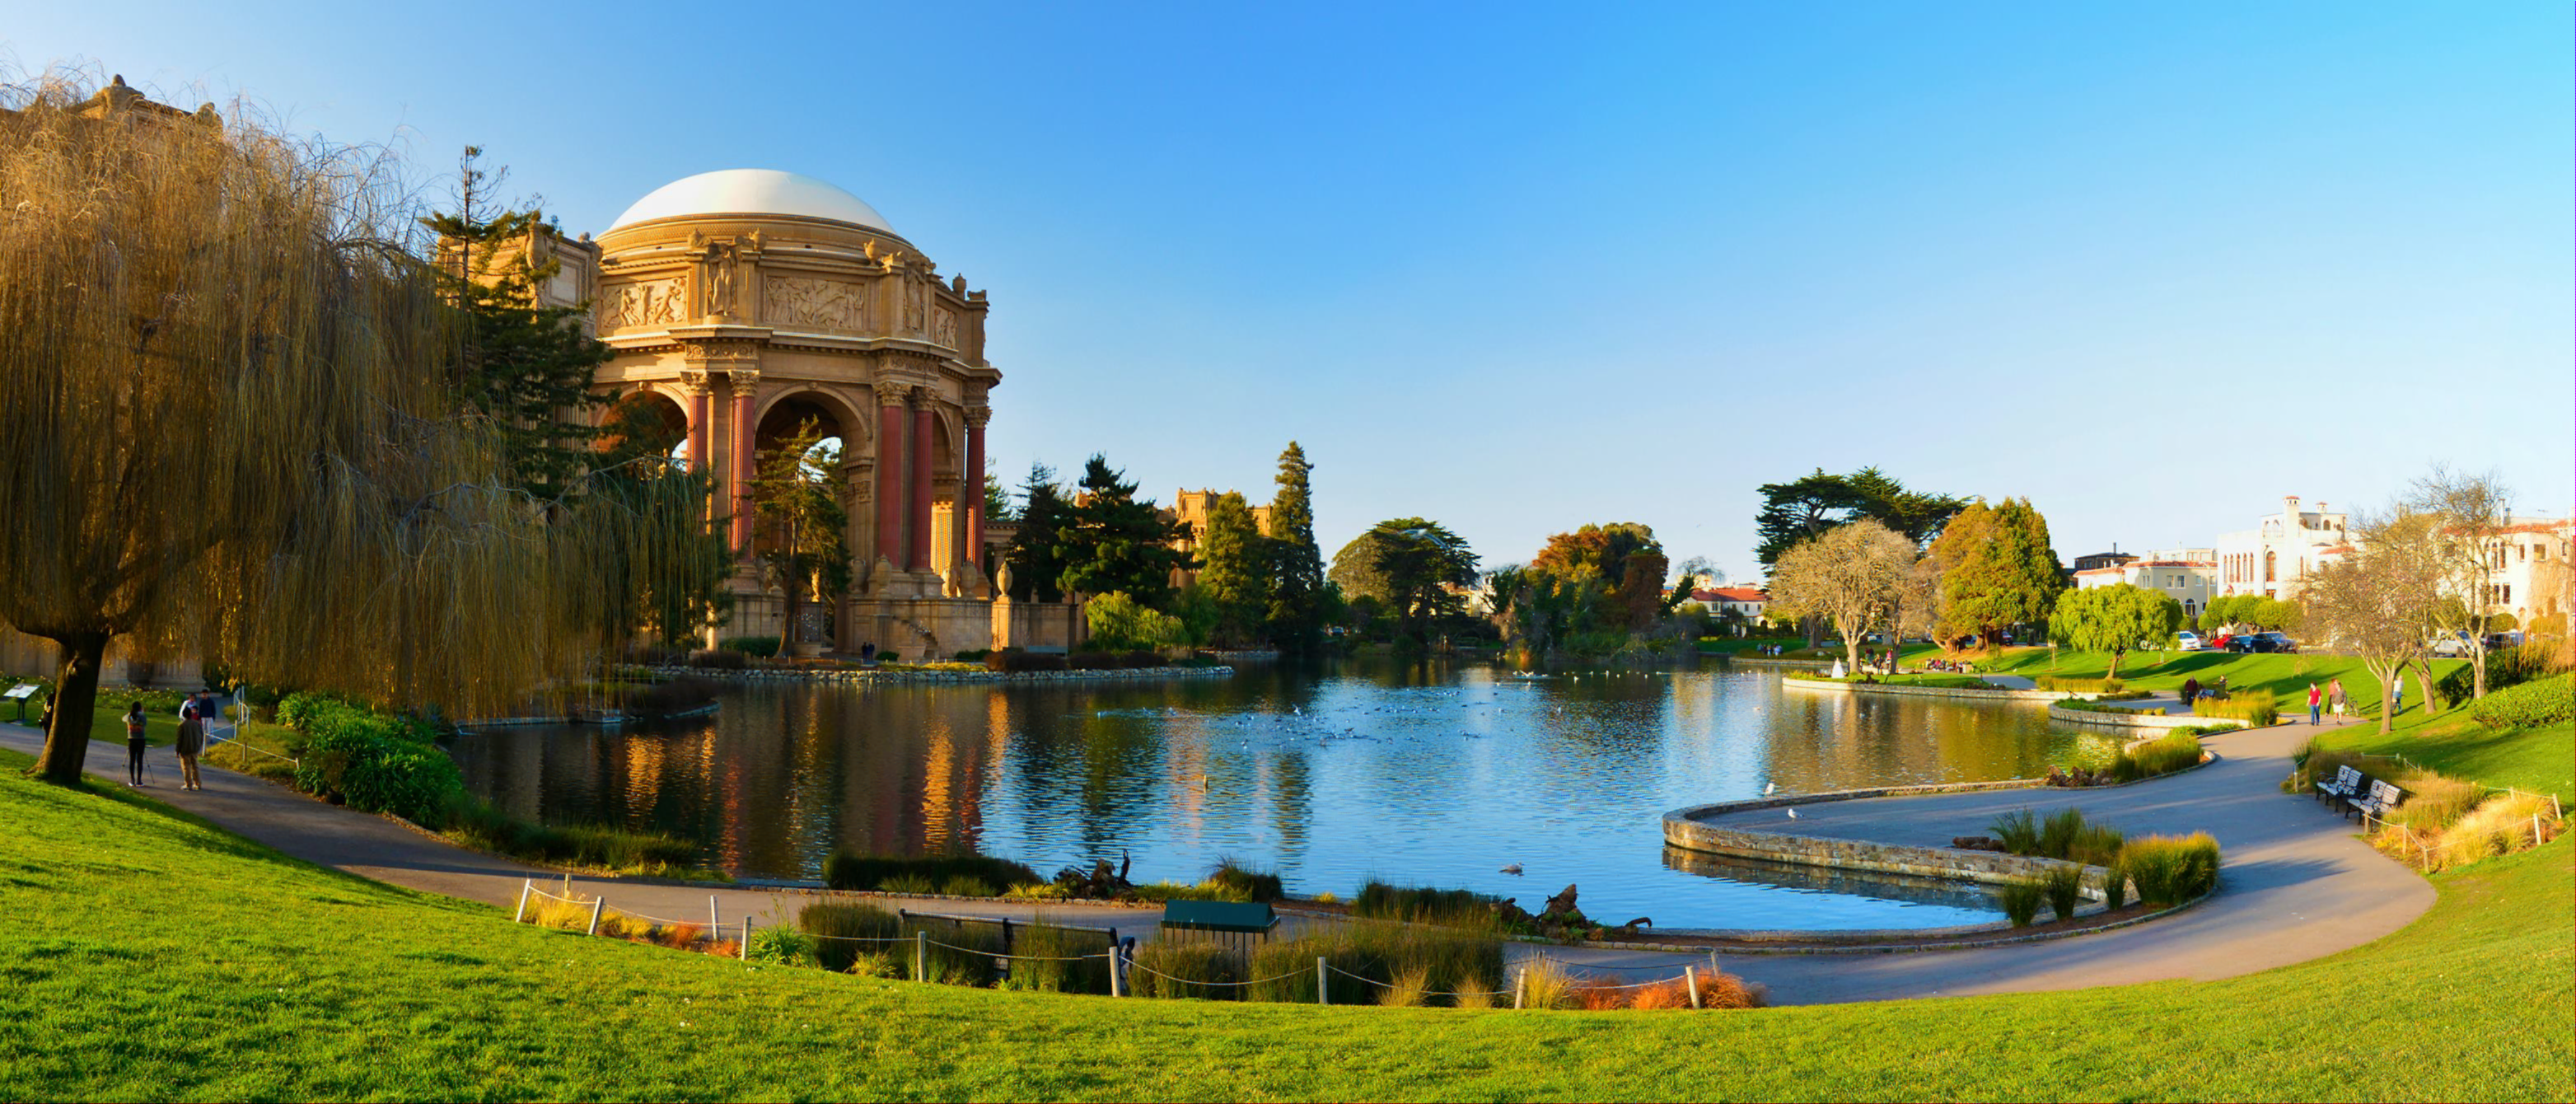
\includegraphics[width=0.95\textwidth]{hw1/problem3/reconstructed.png}
		\caption{Reconstructed image}\label{fig:2c}
	\end{subfigure}
	\caption{Palace of Fine Arts, San Francisco \copyright}\label{fig:2}
\end{figure}


\subsection{Potts Model on Color Images}
Recall the Potts Model that was discussed as a mechanism for modeling piecewise constant images and regularizing region boundaries.
It was shown in the class that how to implement Potts model with loops.
Now you need to implement the Potts model using ideas of \textbf{Spatial Range Map} operators.
The images we are considering here are discrete color images with RGB three channels and for every channel values range from 0 to 255.
You should complete the function \href{./hw1/problem4/potts.m}{\texttt{potts.m}} to return the \(E(I)\) for the given image.
The provided code potts \href{./hw1/problem4/potts_load.m}{\texttt{potts\_load.m}} will load in the images, call \href{./hw1/problem4/potts.m}{\texttt{potts.m}} and display the results for you.
For all code, use \(\beta=1\).
Run and report output figures of \href{./hw1/problem4/potts_load.m}{\texttt{potts\_load.m}}; include your \href{./hw1/problem4/potts.m}{\texttt{potts.m}} verbatim in your pdf submission with brief explanation.
Submit your code together with your report.

\emph{Hint}: the input image is in the format of uint8 and you might need to turn it to double to yield correct answer.


\lstinputlisting[style=Matlab-editor]{./hw1/problem4/potts.m}

In comparison with the previous problem this function is suprisingly short, where there are only 4 lines of effective code (line 12-15).
This is because we use the select row and select column functions to avoid the loop.
The output results are shown in Figure \ref{fig:3}.
The more complex the image is, the larger the entropy is.
Obviously, \ref{fig:3b} has more patterns than \ref{fig:3a}, so it has larger \(E\) .

\begin{figure}[htbp]
	\centering
	\begin{subfigure}[t]{\textwidth}
	    \centering
		\includegraphics[width=0.8\textwidth]{hw1/problem4/i1.pdf}
		\caption{\texttt{I1}, \(E=36\)}\label{fig:3a}
	\end{subfigure}
	\begin{subfigure}[t]{\textwidth}
	    \centering
		\includegraphics[width=0.8\textwidth]{hw1/problem4/i2.pdf}
		\caption{\texttt{I2}, \(E=42\)}\label{fig:3b}
	\end{subfigure}
	\caption{Potts Model of Color Images}\label{fig:3}
\end{figure}